
\section{Improvements For Modelling Non-stationary Sequences}\label{improvinf}
\subsection{Generalized Likelihood Methods}
introduced by \citet{martin_generalized_2000}
As we have seen in \hyperref[likintro]{section \textbf{4.1}}, 
" The ML method may diverge
when sample size is small. To resolve the problems of
divergence occurring in the numerical techniques used for
ML, Martins and Stedinger [2000] suggest the use of a prior
distribution for the shape parameter of the GEV model such
that the most probable values of the parameter are included"

When dealing with nonstationnary processes, it is interesting to consider Generalized Maximum Likelihood (GML) estimators. In this case, \cite{Adlouni_generalized_2007} have proven that GML is likely to outperform the usual ML inference.

The GML estimator corresponds to the mode of the empirical posterior distribution...

\paragraph*{Properties of the GML estimator} see pp740. \citet{martin_generalized_2000}

\section{Neural-Network Based Inference}

\tikzset{%
	neuron missing/.style={
		draw=none, 
		scale=2,
		text height=0.2cm,
		execute at begin node=\color{black}$\vdots$
	},
}
\begin{figure}[!htb]
	\begin{center}
	\resizebox{12cm}{5cm}{ \fbox{
			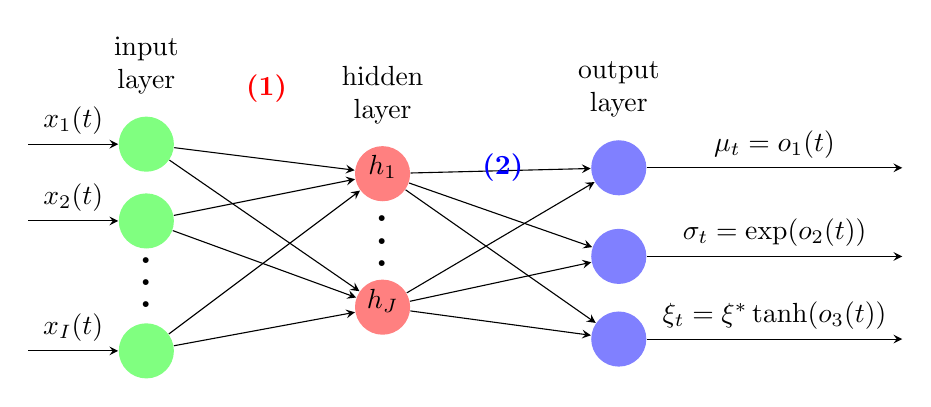
\begin{tikzpicture}[x=1.5cm, y=1.5cm, >=stealth]
			\tikzstyle{annot} = [text width=4em, text centered]
			
			\foreach \m [count=\y] in {1}
			\node [circle,fill=green!50,minimum size=.7cm ] (input-\m) at (0,1) {};
			
			\foreach \m [count=\y] in {2}
			\node [circle,fill=green!50,minimum size=.7cm ] (input-\m) at (0,0.35) {};
			
			\foreach \m [count=\y] in {3}
			\node [circle,fill=green!50,minimum size=.7cm ] (input-\m) at (0,-0.75) {};
			
			\node [neuron missing]  at (0,-0.25) {};
			
			\foreach \m [count=\y] in {1}
			\node [circle,fill=red!50,minimum size=.7cm ] (hidden-\m) at (2,0.75) {};
			
			\foreach \m [count=\y] in {2}
			\node [circle,fill=red!50,minimum size=.7cm ] (hidden-\m) at (2,-0.38) {};
			
			\node [neuron missing]  at (2,0.1) {};
			
			\foreach \m [count=\y] in {1}
			\node [circle,fill=blue!50,minimum size=.7cm ] (output-\m) at (4,1.8-\y) {};
			
			\foreach \m [count=\y] in {2}
			\node [circle,fill=blue!50,minimum size=.7cm ] (output-\m) at (4,1.05-\y) {};
			
			\foreach \m [count=\y] in {3}
			\node [circle,fill=blue!50,minimum size=.7cm ] (output-\m) at (4,0.35-\y) {};
			
			\draw [<-] (input-1) -- ++(-1,0)
			node [above, midway] {$\boldsymbol{x_1(t)}$};
			\draw [<-] (input-2) -- ++(-1,0)
			node [above, midway] {$x_2(t)$};
			\draw [<-] (input-3) -- ++(-1,0)
			node [above, midway] {$x_I(t)$};
			
			\node [below] at (hidden-1.north) {$h_1$};
			\node [below] at (hidden-2.north) {$h_J$};
			
			\draw [->] (output-1) -- ++(2.4,0)
			node [above, midway] {$\boldsymbol{\mu_t=o_1(t)}$};
			\draw [->] (output-2) -- ++(2.4,0)
			node [above, midway] {$\sigma_t=\exp(o_2(t))$};
			\draw [->] (output-3) -- ++(2.4,0)
			node [above, midway] {$\xi_t=\xi^*\tanh(o_3(t))$};
			
			\foreach \i in {1,...,3}
			\foreach \j in {1,...,2}
			\draw [->] (input-\i) -- (hidden-\j);
			
			\foreach \i in {1,...,2}
			\foreach \j in {1,...,3}
			\draw [->] (hidden-\i) -- (output-\j);
			
			\node[annot,above of=hidden-1, node distance=1cm] (hl) {hidden layer};
			\node[annot,above of=input-1] (il) {input layer};
			\node[annot,above of=output-1] {output layer};
			\node[annot, above =2.2cm, right=0.7cm, node distance=1cm]{\textcolor{red}{\textbf{(1)}}};
			\node[annot, above =1.2cm, right=3.7cm]{\textcolor{blue}{\textbf{(2)}}};
			\end{tikzpicture}
		}
	}
	\vspace{-2.5mm}
	\caption{\emph{ Neural Network applied to GEV. Figure made with \texttt{tikzpicture} and based on  \textcolor{JungleGreen}{\cite{cannon_flexible_2010}}} }
	\end{center}
\end{figure}

\paragraph*{Parametric or nonparametric ?}
It is always a difficult task to state whether Neural Networks (NN) are parametric models or not. NN  are somewhere in the gray area between a \emph{parametric} and a \emph{nonparametric} model, in the sense that it assumes the GEV distribution from the output layer which are defined by the three parameters of interest, while it also allows for a fabulous flexibility coming from the hidden layers and which lead to think that these ae rather nonparametric.
However, this terminological question is actually not relevant here and it is more important to focus on the model of NN that is employed here.

have the power to manage several outputs in a 

"Model parameters are estimated via the GML approach using the
quasi-Newton BFGS optimization algorithm, and the appropriate GEV-CDN model architecture for
each location is selected by fitting increasingly complicated models and choosing the one that
minimizes appropriate cost-complexity model selection criteria. For each location examined, different
formulations are tested with combinational cases of stationary and nonstationary parameters of the
GEV distribution, linear and nonlinear architecture of the CDN and combinations of the input covariates "


\cite{carreau_hybrid_2009} enlightens the following : Provided enough data, hidden units and an appropriate optimization, the NN can capture any smooth dependencies (relationships) of the parameters on the input, i.e., given the input, it can theoretically capture any conditional continuous density, be it asymmetric, \textbf{multimodal}, or heavy-tailed.

(see \citet{cannon_flexible_2010} just before conclusion) 
One could for example expect to have particular relationships between the covariate (time or) and the parameters of interest. Only considering a linear or quadratic trends in the location parameter $\mu$ (ore more ? see section. see for other parameters) could thus be seen as a weak modelling procedure, especially when we assumed no reliable prior knowledge on the subject (see bayesian section - hyperref it).
NN models have this facility of being capable of modelling any relationships without explicitly specify it \emph{a priori}. To model correctly, one should be able to explicitly discover particular patterns (e.g., which nonlinear or linear relationship between time and TN). This is avoided here because this is done automatically through the NN process.

Physical process such as temperature or even other meteorological data (rainfall as demonstrated by \citet{cannon_flexible_2010},...) have this tendance of demonstrating nonlinearities ( see ref?) and so are NN's interesting.

As we mentioned, the NN is meant to approximate any functions with good accuracy. It comprise thus all the models considered so far, such as linear tren din $\mu$, quadratic, etc...

\citet{cannon_flexible_2010} recommended to use between 1 and 3 (4) hidden layers due to the relatively small sample of annual extremes (here 117).


 From this, we must pay attention to the high danger of \emph{overfitting} (see ) which occurs for this sort of models. The other pitfall is its lack of interpretation of the retrieved relationships.
 
 "It bears noting that sensitivity analysis methods,
 for example, the one used by Cannon and McKendry
 (2002), are applicable to CDN models and could be used
 to identify the form of nonlinear relationships between
 covariates and GEV distribution parameters or quantiles."
 
 ... Intro to deep learning.. ?
 
\section{Bagging} 

Nowadays, bagging is used in 
many state-of-the-art algorithms such as Random Forests (see .. for comparisons of such techniques) and is one of the \emph{ensemble methods} which are praised in Machine Learning for their performance.  

In a "pure" climatological point of view, \emph{ensemble models} are of major utility, especially to make weather forecasting, see for example \citet{suh_development_2012} or, .... among others

For our purpose, we present another kind of ensemble modelling which is \emph{bagging}.

" Bagging (stands for Bootstrap Aggregation) is the way decrease the variance of your prediction by generating additional data for training from your original dataset using combinations with repetitions to produce multisets of the same cardinality/size as your original data. By increasing the size of your training set you can't improve the model predictive force, but just decrease the variance, narrowly tuning the prediction to expected outcome "


"model averaging, which involves taking a weighted average of
multiple models, has been recommended as a means of
improving estimation performance Burnham and Anderson, 2004. This approach has been applied successfully
in the context of CDN models by Carney et al. (2005)
and is worth exploring for GEV-CDN models."


\citet[pp.256-267]{Goodfellow-et-al-2016}  (deep learning html book)    The  individual  classifiers’  predictions  (having
equal  weightage)  are  then  combined  by  taking  majority voting. This typically reduces the variance and then the (possible) overfitting






\section{Bootstrap Methods in EVT}

" like
the estimated parameters themselves, the SE may not be
reliable for small samples. One way to tackle this problem and improve the accuracy of SE is through the bootstrap technique (Efron, 1979). The scheme for using this technique for EV distribution  function is described in detail by Katz et al. (2002), including for nonstationary cases,
in which the bootstrap samples are manufactured through
Monte  Carlo  resampling  of  residuals  (Equation (8))  to attend  to  the  underlying  assumption  that  original  sam-
ple  consist  of  iid  data.  Following  this procedure,  the bootstrap  procedure  was  designed  for  generating  1000
samples  from  each  original  sample,  considering  whole year  as  a  bloc"


In \citet{cannon_flexible_2010}, "he parametric bootstrap outperformed the residual bootstrap"
Moreover, " It is possible that alternative bootstrap approaches, for example, the bias-adjusted percentile estimators evaluated by Kysely
(2008), might yield better calibrated confidence intervals, although improvements were modest for stationary GEV models. "


For confidence intervals : see \citet[pp.681]{cannon_flexible_2010} 
following these steps

\begin{enumerate}
	\item Fit a nonstationary model to the data
	\item Transform the residuals from the fitted model so that they are identically distributed :
	\begin{equation}
	\varepsilon_t=\bigg[1+\xi_t\sigma^{-1}_t(y_t-\mu_t)\bigg]^{-\xi^{-1}}
	\end{equation}
	\item etc..
\end{enumerate}

Monte-Carlo based methods, same as Bayesian.

Study and comparisons on the performance (coverage,..) of the methods used for the CI (boot, bayesian, likelihood, asymptotics,...)
\subsection{Moving Block Bootstrap}

[Bootstrap and other resampling in .... pp.13]


\section{Markov models}
book risk pp.136, \cite{shaby_markov-switching_2016} + code


